% !TEX encoding = UTF-8
% !TEX program = xelatex
\documentclass[12pt,a4paper]{article}
\usepackage[paperwidth=210mm, paperheight=297mm, left=0.75in, right=0.75in, bottom=1in, top=1in]{geometry}
\usepackage{polyglossia}
\setdefaultlanguage[babelshorthands]{italian}
\usepackage{fontspec}
\usepackage{graphicx}
\usepackage{blindtext}
\usepackage{wrapfig}

\frenchspacing
\makeindex

\begin{document}
\title{\vspace{-70pt}Copernicus (OAO 3)}
\author{Nicola Sarassi}
\date{}
\maketitle
\pagestyle{empty}
\thispagestyle{empty}

\section*{Storia}
\label{storia}
\begin{wrapfigure}{r}{0.35\textwidth}
  \vspace{-10pt}
  \begin{center}
    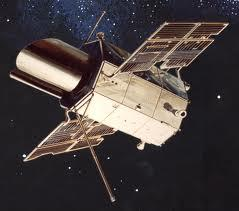
\includegraphics[width=0.30\textwidth]{satellite}
  \end{center}
  \vspace{-20pt}
\end{wrapfigure}
Fu lanciato il 21 agosto 1972 e fu chiamato Copernico perché ricorreva il 500º anniversario della nascita di Niccolò Copernico. Il satellite venne lanciato dalla NASA, ma la missione fu effettuata in collaborazione tra istituzioni scientifiche degli USA e del Regno Unito. Il satellite era equipaggiato con un telescopio per l'ultravioletto con un diametro di 80 cm e un rilevatore di raggi X. Il satellite Copernico operò fino al febbraio 1981 ed effettuò centinaia di osservazioni. Permise di scoprire parecchie stelle pulsar a lungo periodo, cioè con periodi di rotazione di molti minuti anziché di pochi secondi come normalmente avviene.

\section*{Osservazioni}
\label{osservazioni}

I pannelli solari sono stati fissati con un angolo di 34 gradi rispetto all'asse di osservazione del telescopio, e sono stati mantenuti entro i 30 gradi del Sole. Questa limitazione ha determinato la visione di alcune parti del cielo che sono visibili solo in alcune parti dell'anno. Gli strumenti astronomici sono stati co-allineati, con il telescopio UV residente nel cilindro centrale del satellite. 

\end{document}